%!TEX TS-program = xelatex

% Шаблон документа LaTeX создан в 2018 году
% Алексеем Подчезерцевым
% В качестве исходных использованы шаблоны
% 	Данилом Фёдоровых (danil@fedorovykh.ru) 
%		https://www.writelatex.com/coursera/latex/5.2.2
%	LaTeX-шаблон для русской кандидатской диссертации и её автореферата.
%		https://github.com/AndreyAkinshin/Russian-Phd-LaTeX-Dissertation-Template

\documentclass[a4paper,14pt]{article}


%%% Работа с русским языком
\usepackage[english,russian]{babel}   %% загружает пакет многоязыковой вёрстки
\usepackage{fontspec}      %% подготавливает загрузку шрифтов Open Type, True Type и др.
\defaultfontfeatures{Ligatures={TeX},Renderer=Basic}  %% свойства шрифтов по умолчанию
\setmainfont[Ligatures={TeX,Historic}]{Times New Roman} %% задаёт основной шрифт документа
\setsansfont{Comic Sans MS}                    %% задаёт шрифт без засечек
\setmonofont{Courier New}
\usepackage{indentfirst}
\frenchspacing

\renewcommand{\epsilon}{\ensuremath{\varepsilon}}
\renewcommand{\phi}{\ensuremath{\varphi}}
\renewcommand{\kappa}{\ensuremath{\varkappa}}
\renewcommand{\le}{\ensuremath{\leqslant}}
\renewcommand{\leq}{\ensuremath{\leqslant}}
\renewcommand{\ge}{\ensuremath{\geqslant}}
\renewcommand{\geq}{\ensuremath{\geqslant}}
\renewcommand{\emptyset}{\varnothing}

%%% Дополнительная работа с математикой
\usepackage{amsmath,amsfonts,amssymb,amsthm,mathtools} % AMS
\usepackage{icomma} % "Умная" запятая: $0,2$ --- число, $0, 2$ --- перечисление

%% Номера формул
%\mathtoolsset{showonlyrefs=true} % Показывать номера только у тех формул, на которые есть \eqref{} в тексте.
%\usepackage{leqno} % Нумерация формул слева	

%% Перенос знаков в формулах (по Львовскому)
\newcommand*{\hm}[1]{#1\nobreak\discretionary{}
	{\hbox{$\mathsurround=0pt #1$}}{}}

%%% Работа с картинками
\usepackage{graphicx}  % Для вставки рисунков
\graphicspath{{images/}}  % папки с картинками
\setlength\fboxsep{3pt} % Отступ рамки \fbox{} от рисунка
\setlength\fboxrule{1pt} % Толщина линий рамки \fbox{}
\usepackage{wrapfig} % Обтекание рисунков текстом

%%% Работа с таблицами
\usepackage{array,tabularx,tabulary,booktabs} % Дополнительная работа с таблицами
\usepackage{longtable}  % Длинные таблицы
\usepackage{multirow} % Слияние строк в таблице
\usepackage{float}% http://ctan.org/pkg/float

%%% Программирование
\usepackage{etoolbox} % логические операторы


%%% Страница
\usepackage{extsizes} % Возможность сделать 14-й шрифт
\usepackage{geometry} % Простой способ задавать поля
\geometry{top=20mm}
\geometry{bottom=20mm}
\geometry{left=20mm}
\geometry{right=10mm}
%
%\usepackage{fancyhdr} % Колонтитулы
% 	\pagestyle{fancy}
%\renewcommand{\headrulewidth}{0pt}  % Толщина линейки, отчеркивающей верхний колонтитул
% 	\lfoot{Нижний левый}
% 	\rfoot{Нижний правый}
% 	\rhead{Верхний правый}
% 	\chead{Верхний в центре}
% 	\lhead{Верхний левый}
%	\cfoot{Нижний в центре} % По умолчанию здесь номер страницы

\usepackage{setspace} % Интерлиньяж
\onehalfspacing % Интерлиньяж 1.5
%\doublespacing % Интерлиньяж 2
%\singlespacing % Интерлиньяж 1

\usepackage{lastpage} % Узнать, сколько всего страниц в документе.

\usepackage{soul} % Модификаторы начертания

\usepackage{hyperref}
\usepackage[usenames,dvipsnames,svgnames,table,rgb]{xcolor}
\hypersetup{				% Гиперссылки
	unicode=true,           % русские буквы в раздела PDF
	pdftitle={Автоматизация проектных работ},   % Заголовок
	pdfauthor={Солодянкин А.А.},      % Автор
	pdfsubject={Автоматизация проектных работ},      % Тема
	pdfcreator={Солодянкин А.А.}, % Создатель
	pdfproducer={Солодянкин А.А.}, % Производитель
	pdfkeywords={Автоматизация проектных работ}, % Ключевые слова
	colorlinks=true,       	% false: ссылки в рамках; true: цветные ссылки
	linkcolor=black,          % внутренние ссылки
	citecolor=black,        % на библиографию
	filecolor=magenta,      % на файлы
	urlcolor=black           % на URL
}
\makeatletter 
\def\@biblabel#1{#1. } 
\makeatother
\usepackage{cite} % Работа с библиографией
%\usepackage[superscript]{cite} % Ссылки в верхних индексах
%\usepackage[nocompress]{cite} % 
\usepackage{csquotes} % Еще инструменты для ссылок

\usepackage{multicol} % Несколько колонок

\usepackage{tikz} % Работа с графикой
\usepackage{pgfplots}
\usepackage{pgfplotstable}

% ГОСТ заголовки
\usepackage[font=small]{caption}
%\captionsetup[table]{justification=centering, labelsep = newline} % Таблицы по правобу краю
%\captionsetup[figure]{justification=centering} % Картинки по центру


\newcommand{\tablecaption}[1]{\addtocounter{table}{1}\small \begin{flushright}\tablename \ \thetable\end{flushright}%	
\begin{center}#1\end{center}}

\newcommand{\imref}[1]{рис.~\ref{#1}}

\usepackage{multirow}
\usepackage{spreadtab}
\newcolumntype{K}[1]{@{}>{\centering\arraybackslash}p{#1cm}@{}}


\usepackage{xparse}
\usepackage{fancyvrb}

\RecustomVerbatimCommand{\VerbatimInput}{VerbatimInput}
{
	fontsize=\footnotesize    
}

\newcolumntype{?}[1]{!{\vrule width #1}}

\usepackage{tocloft}
\renewcommand{\cftsecleader}{\cftdotfill{\cftdotsep}}
\begin{document} % конец преамбулы, начало документа
\begin{titlepage}
	\begin{center}
		ПРАВИТЕЛЬСТВО РОССИЙСКОЙ ФЕДЕРАЦИИ \\
 		ФЕДЕРАЛЬНОЕ  ГОСУДАРСТВЕННОЕ АВТОНОМНОЕ \\
		ОБРАЗОВАТЕЛЬНОЕ УЧРЕЖДЕНИЕ ВЫСШЕГО ОБРАЗОВАНИЯ\\
		«НАЦИОНАЛЬНЫЙ ИССЛЕДОВАТЕЛЬСКИЙ УНИВЕРСИТЕТ\\
		«ВЫСШАЯ ШКОЛА ЭКОНОМИКИ»
	\end{center}
	
	\begin{center}
		\textbf{Московский институт электроники и математики}
		
		\textbf{Им. А.Н.Тихонова НИУ ВШЭ}
		
		\vspace{2ex}
		
		\textbf{Департамент компьютерной инженерии}
	\end{center}
	\vspace{1ex}	
	
	\vspace{1ex}
	\begin{center}
		\textbf{Практическая работа №3 \\
			«Знакомство с САПР Altera Quartus II» \\
			Вариант №13
	}
	\end{center}	

	\vspace{2ex}
	\vfill
	
	\vspace{2ex}
	
	\begin{flushright}
		\textbf{Выполнил:}
		
		\vspace{2ex}
		
		Студент группы БИВ174
		
		\vspace{2ex}
		
		Солодянкин Андрей Александрович
		
		\vspace{2ex}
		
		\textbf{Проверил:}
		
		\vspace{2ex}
		
		Романова Ирина Ивановна
	\end{flushright}

	\vspace{5ex}
	\begin{center}
		Москва \the\year \, г.
	\end{center}
	
\end{titlepage}
\addtocounter{page}{1}

\tableofcontents
\pagebreak

\section{Цель работы}

Моделирование работы дешифратора, изучение карт Карно.

\section{Задание}

\begin{itemize}
	\item Вариант -- 13;
	
	\item Начало диапазона -- 0xC38;
	
	\item Конец диапазона -- 0xC3E;
	
	\item Исключение -- 0x3CA, 0x3CB;
\end{itemize}

\begin{enumerate}
\item Создать схему для проверки функции дешифратора и произвести замер временных задержек.

\item Запрограммировать учебную плату и продемонстрировать результаты работы на макете.

\item Построить временную диаграмму и выполнить моделирование в режимах Functional и Time. Сравнить и обосновать полученные результаты.
\end{enumerate}



\section{Выполнение работы}

\subsection{Вывод формулы}

Переведем шестнадцатеричные значения в их двоичные преставления

0x3C8 = 0011 1100 1000

0x3CA = 0011 1100 1010

0x3CB = 0011 1100 1011

0x3CE = 0011 1100 1110

У всех значений общая часть первые 9 битов, для остальных трех запишем таблицу истинности (таблица \ref{tab:ist}) и по ней составим карту Карно (таблица \ref{tab:karno}).

\begin{table}[H]
	\caption{Таблица истинности}	
	\label{tab:ist}
	\begin{center}
		\begin{tabular}{|l|l|l|l|}
			\hline
			$X_2$ & $X_1$ & $X_0$ & $Y$ \\ \hline
			0 & 0 & 0 & 1 \\ \hline
			0 & 0 & 1 & 1 \\ \hline
			0 & 1 & 0 & 0 \\ \hline
			0 & 1 & 1 & 0 \\ \hline
			1 & 0 & 0 & 1 \\ \hline
			1 & 0 & 1 & 1 \\ \hline
			1 & 1 & 0 & 1 \\ \hline
			1 & 1 & 1 & 0 \\ \hline
		\end{tabular}
	\end{center}
\end{table}

\begin{table}[H]
	\caption{Карта Карно}	
	\label{tab:karno}
	\begin{center}
		\begin{tabular}{c|c|c|c|c|}
			& \multicolumn{2}{c|}{$X_2$}     & \multicolumn{2}{c|}{$\overline X_2$}    \\ \hline
			$X_1$           & 1                 & 0        & 0             & 0                     \\ \hline
			$\overline X_1$ & 1                 & 1        & 1             & 1                     \\ \hline
			& $\overline X_0$     & \multicolumn{2}{c|}{$X_0$} & $\overline X_0$        
		\end{tabular}
	\end{center}
\end{table}

Получим минимизированную функцию из карты Карно, формула \ref{f:f1}.

\begin{equation}
\label{f:f1}
\begin{gathered}
F_{012} = \overline X_1 + X_2 * \overline X_0 
\end{gathered}
\end{equation}

Итоговый результат дешифратора можно выразить через формулу \ref{f:f2}.

\begin{equation}
\label{f:f2}
\begin{gathered}
F_{itog} = \overline X_{11} * \overline X_{10} * X_9 * X_8 * X_7 * X_6 * \overline X_5 * \overline X_4 * X_3 * (\overline X_1 + X_2 * \overline X_0)
\end{gathered}
\end{equation}

\subsection{Составление программы}

	\begin{figure}[H]
		\centering
		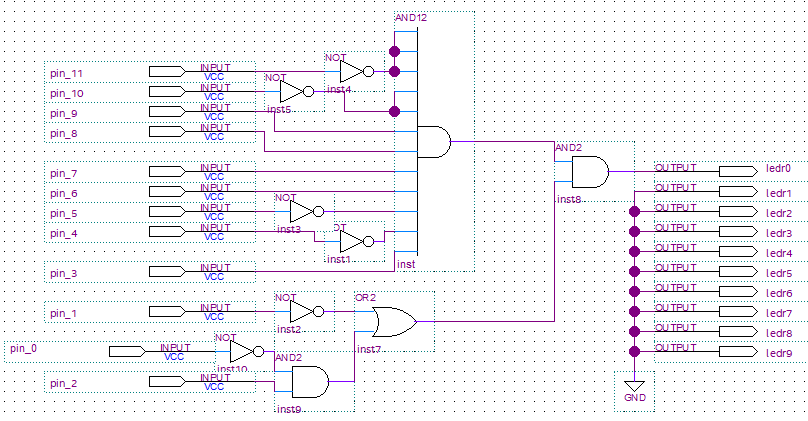
\includegraphics[width=0.7\linewidth]{image/03_bdf}
		\caption{bdf представление итоговой функции дешифратора}
		\label{fig:03bdf}
	\end{figure}

	\begin{figure}[H]
		\centering
		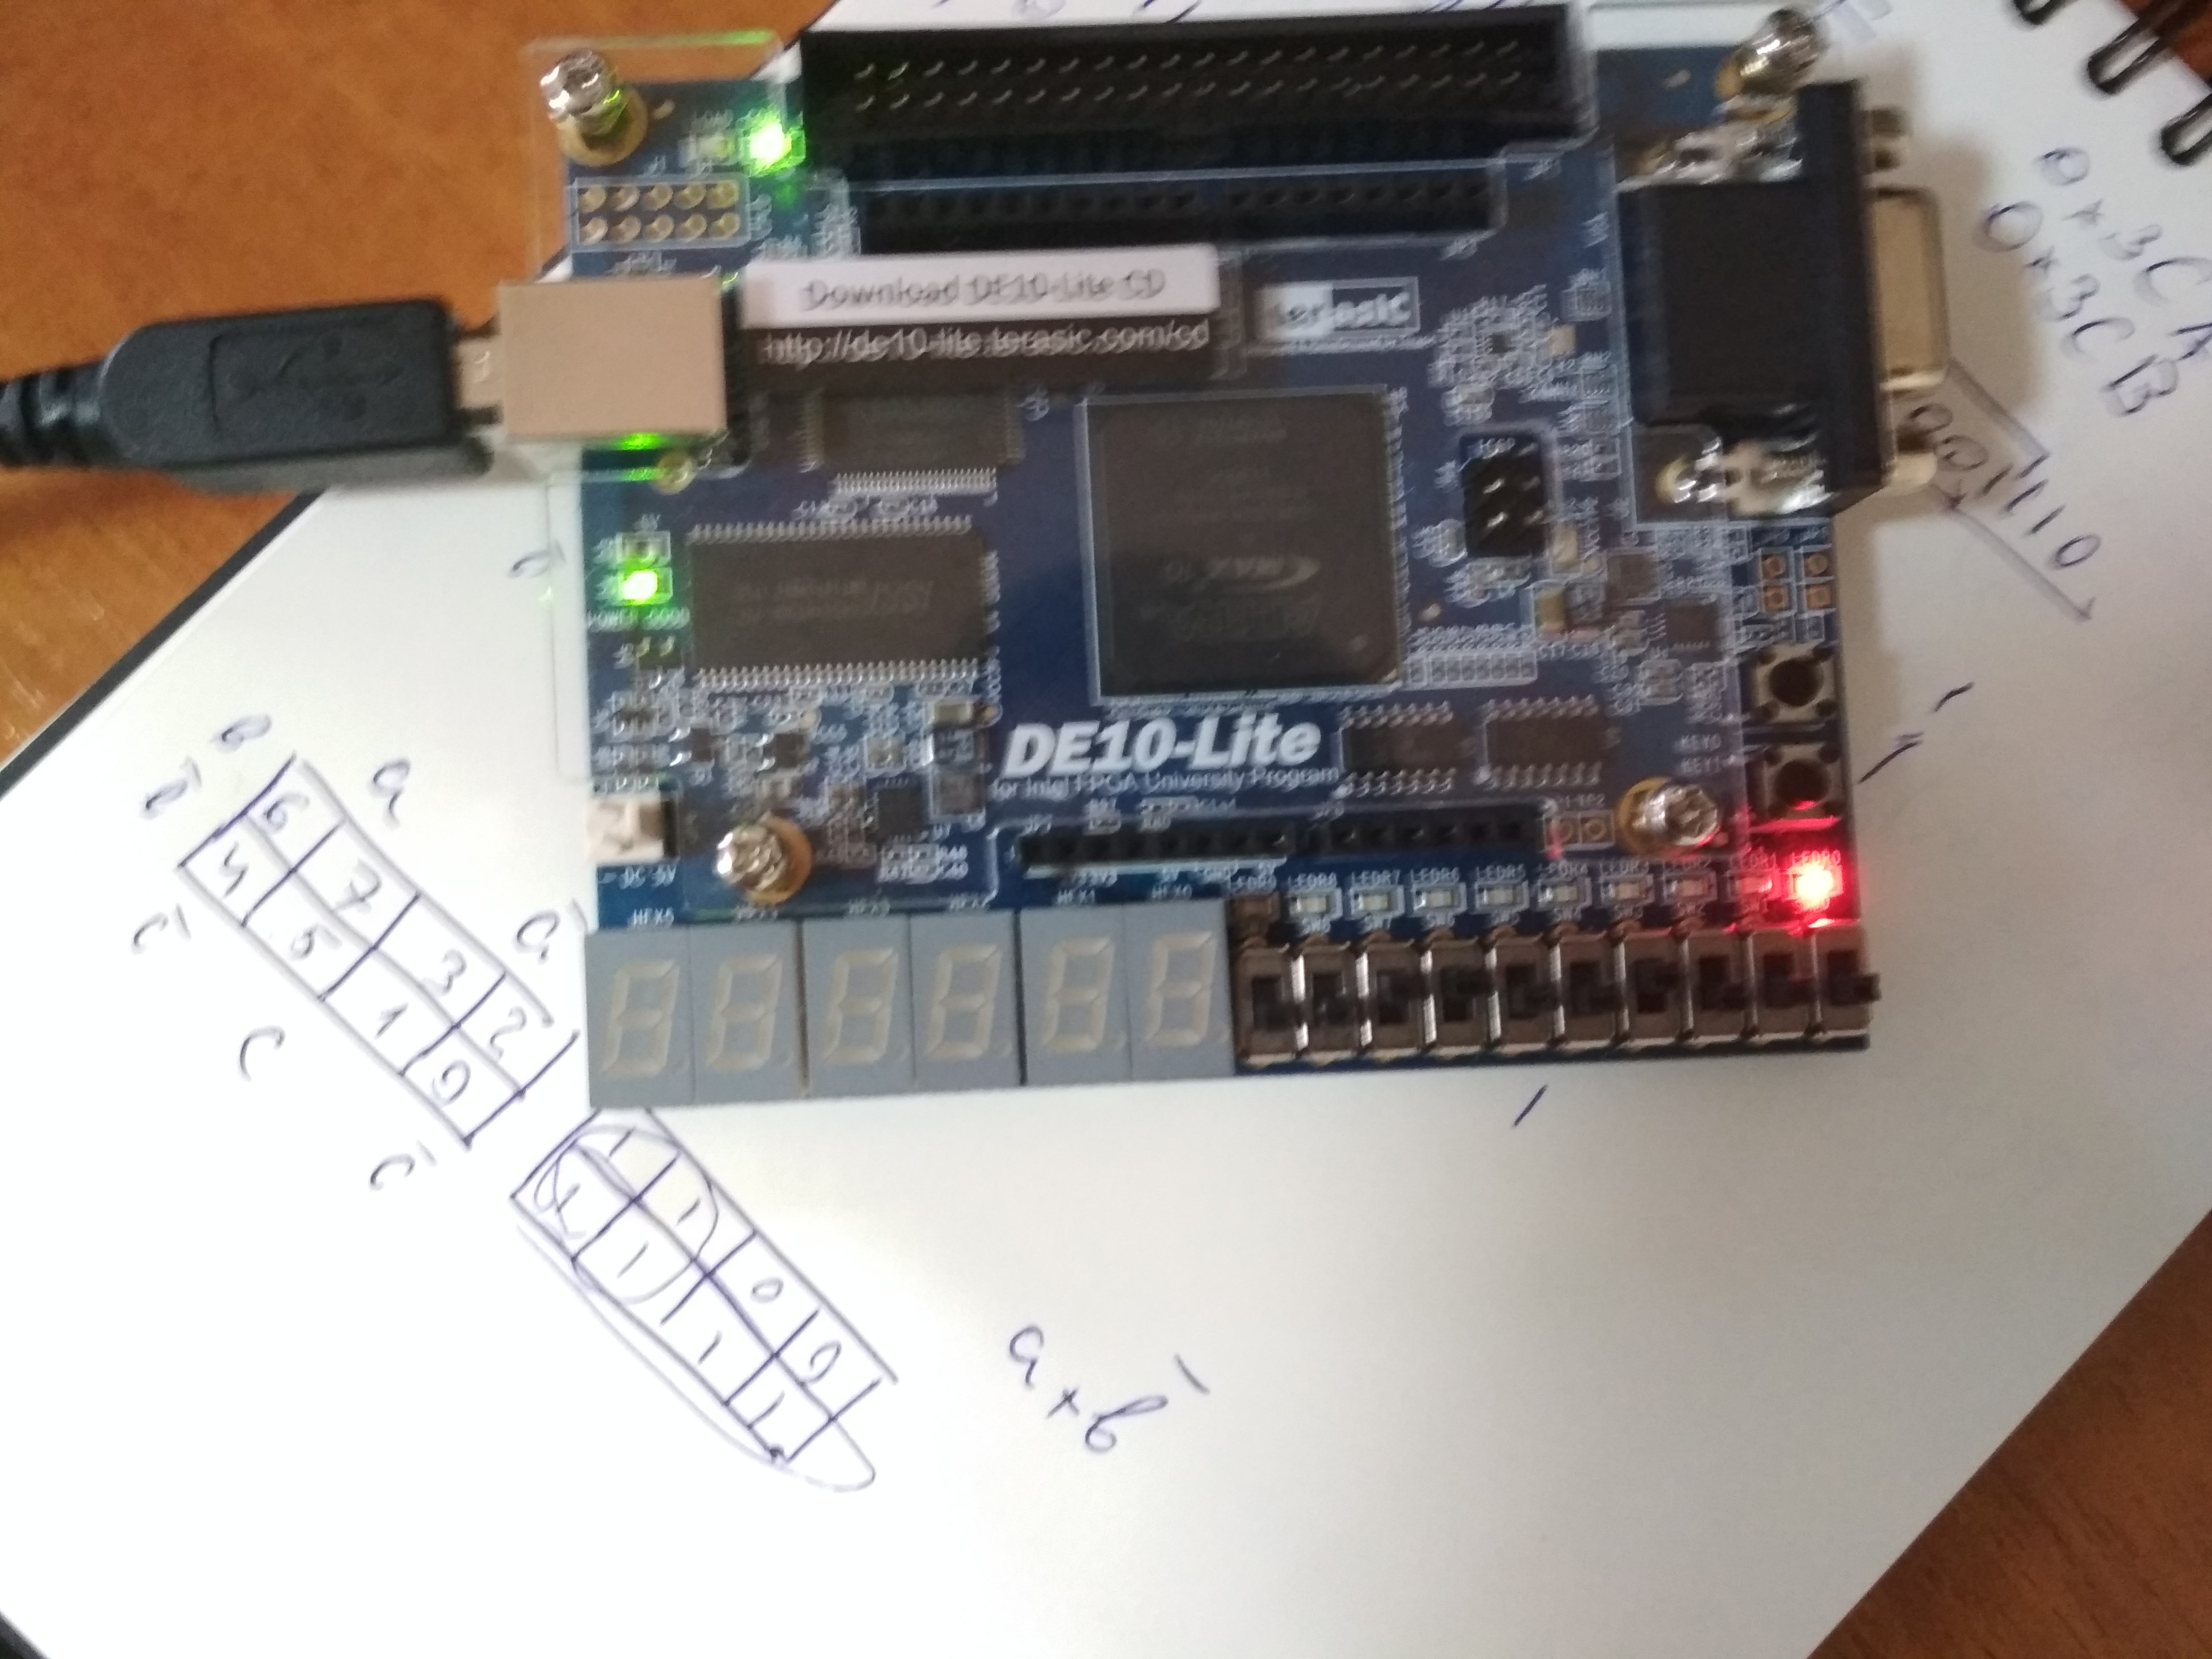
\includegraphics[width=0.7\linewidth]{image/03_foto.JPG}
		\caption{фото рабочей платы}
		\label{fig:03foto}
	\end{figure}

\subsection{Тестирование программы}

	\begin{figure}[H]
		\centering
		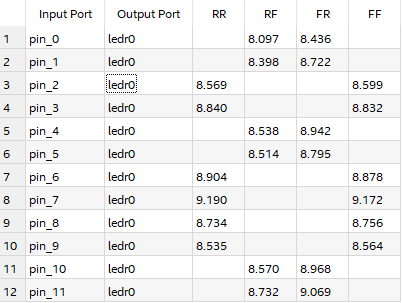
\includegraphics[width=0.7\linewidth]{image/03_times}
		\caption{Временные задержки}
		\label{fig:03times}
	\end{figure}

	Временные задержки (рис. \ref{fig:03times}) были получены следующим образом:
	TimeQuest Timing Analysis > Write SDC file.. > Report Datasheet.

	\begin{figure}[H]
		\centering
		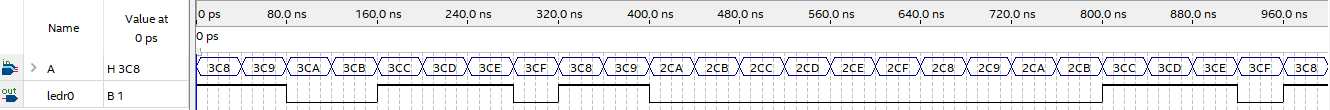
\includegraphics[width=1\linewidth]{image/03_wvf}
		\caption{Временная диаграмма Functional}
		\label{fig:03wvf}
	\end{figure}

	\begin{figure}[H]
		\centering
		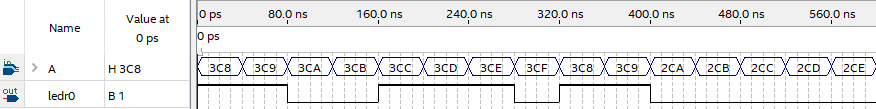
\includegraphics[width=1\linewidth]{image/03_wvf1}
		\caption{Временная диаграмма Time}
		\label{fig:03wvf1}
	\end{figure}


 Моделирование в режимах Functional и Time не отличается, т.к. на приведенной частоте задержек не видно.

\section{Вывод}
В ходе проделанной работы был создан дешифратор, принимающий сигналы в определенных границах с исключениями.
Для минимизации были использованы карты Карно.
При помощи TimeQuest Timing Analysis были получены задержки для кажого входного параметра.
Схема была протестированы при помощи WaneForm, а также удалось загрузить схему на плату и протестировать работоспособность программы на плате.

\newpage 
\renewcommand{\refname}{{\normalsize СПИСОК ИСПОЛЬЗОВАННЫХ ИСТОЧНИКОВ}} 
\centering 
\begin{thebibliography}{9} 
	\addcontentsline{toc}{section}{\refname} 
	\bibitem{sql} Vijayakumar P., Vijayalakshmi V., Zayaraz G. Comparative study of hyperelliptic curve cryptosystem over prime field and its survey //International Journal of Hybrid Information Technology. – 2014. – Т. 7. – №. 1. – С. 137-146.
	\bibitem{sql} Антонов А., Филиппов А., Золотухо Р. Средства системной отладки САПР Quartus II //Компоненты и технологии. – 2008. – №. 89.
\end{thebibliography}

\end{document} % конец документа